\subsection{Расчет скоростей слабых распадов} \label{sec:weakfit}

  Помимо реакций нейтронного захвата, важную роль в $r$-процессе играют $\beta^-$-распады. Скорость слабых распадов сильно зависит массы распадающегося и конечного ядер, на что указывает хорошо известное соотношение Сарджента $\lambda \sim Q^5$, связывающее скорость распада $\lambda$ с энерговыделением $Q$. Для учета влияния выбора массовой модели на распределение продуктов $r$-процесса следовало бы рассчитывать скорости не только реакции $(n,\gamma)$, но и $\beta$-распадов, варьируя массовую модель. Для расчета периодов $\beta$-распадов применяются различные теоретические модели: ССЫЛКА НА МОДЕЛИ. В ряде работ были представлены наборы данных по скоростям $\beta$-распада для большой совокупности ядер: ССЫЛКА НА ПУБЛИКАЦИИ, НАЙТИ ЧЕРЕЗ РЕАКЛИБ И ПАНОВА. Данные из работы ТАКОЙ-ТО были включены в базу данных REACLIB, которая используется в данной работе.

  После проведения расчета скоростей реакций нейтронного захвата на ядрах, входящих в используемые в настоящей работе таблицы теоретических масс, оказалось, что в REACLIB отсутствуют скорости слабых распадов для некоторых ядер-продуктов.  Обусловлено это тем, что разные ядерные модели по-разному предсказывают не только энергии связи, но и область существования яде, определяемые знаком энергий отделения протона $B_p$ и нейтрона $B_n$:
  \begin{equation}\begin{aligned}\label{eq:driplines}
    B_p(A,Z) &= E_{\text{св}}(A,Z) - E_{\text{св}}(A-1,Z-1),\\
    B_n(A,Z) &= E_{\text{св}}(A,Z) - E_{\text{св}}(A-1,Z)
  \end{aligned}\end{equation},
  где $E_{\text{св}}$ --- энергия связи ядра, зависящая от выбора массовой модели. При отрицательных значениях $B_p$ или $B_n$ протон или нейтрон, соответственно, будет беспрепятственно покидать ядро. Ясно, что положение линии отделения нейтрона должно существенно влиять на протекание $r$-процесса, потому что в области $B_n < 0$ накопление нейтронов становится невозможным.

  На рис.~\ref{img:weak_comparison} синим цветом отмечены ядра, для которых в REACLIB присутствуют данные по слабым распадам, а оранжевым --- отсутствующие в REACLIB ядра, являющиеся продуктами рассчитанных нами с помощью модели HFB-24 реакций $(n,\gamma)$. Если добавить такие реакции $(n,\gamma)$ в REACLIB без соответствующих распадов, то их продукты будут накапливаться, приводя к некорректным результатам моделирования $r$-процесса.

  Отметим, что в условиях астрофизического $r$-процесса по его определению характерные времена $\beta^-$-распадов превышают скорости реакции $(n,\gamma)$ на порядки. Таким образом для достижения удовлетворительной точности симуляции $r$-процесса, в особенности на коротких промежутках времени около $1$~с, достаточно задать скорости слабых распадов приблизительно. Поэтому было принято решение не менять скорости тех $\beta^-$-распадов, которые уже присутствовали в REACLIB, а недостающие получить с помощью экстраполяции.
  
\begin{figure}
  \centering
  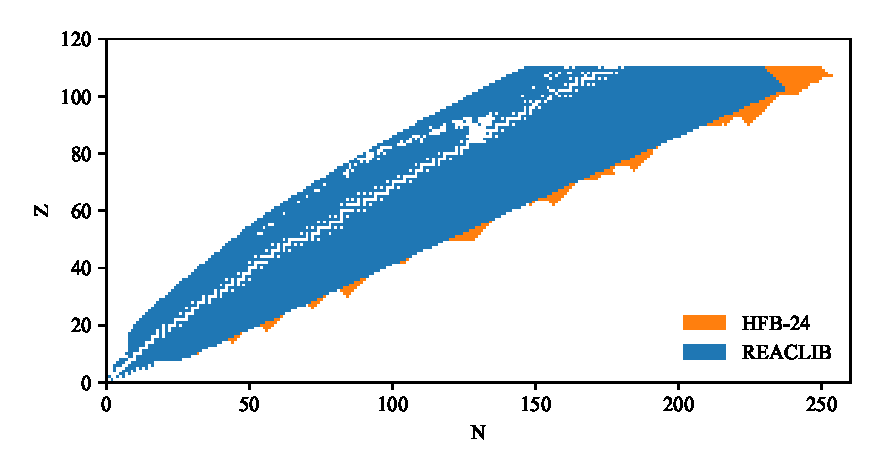
\includegraphics[width=0.8\textwidth]{pics/chart_weak_comparison.eps}
  \caption{Данные о слабых распадах из библиотеки REACLIB (синие квадраты) и нейтроноизбыточные изотопы, присутствующие в таблице масс HFB-24, но отсутствующие в REACLIB (оранжевые квадраты).}
  \label{img:weak_comparison}
\end{figure}
 
\begin{figure}
  \centering
  %\begin{subfigure}{0.48\textwidth}
  %  \centering
  %  \includegraphics[width=\textwidth]{pics/decay_fit26.pdf}
  %  \caption{Железо}
  %\end{subfigure}
  %\hfill
  \begin{subfigure}{0.48\textwidth}
    \centering
    \includegraphics[width=\textwidth]{pics/decay_fit65.pdf}
    \caption{Тербий}
  \end{subfigure}
  \hfill
  \begin{subfigure}{0.48\textwidth}
    \centering
    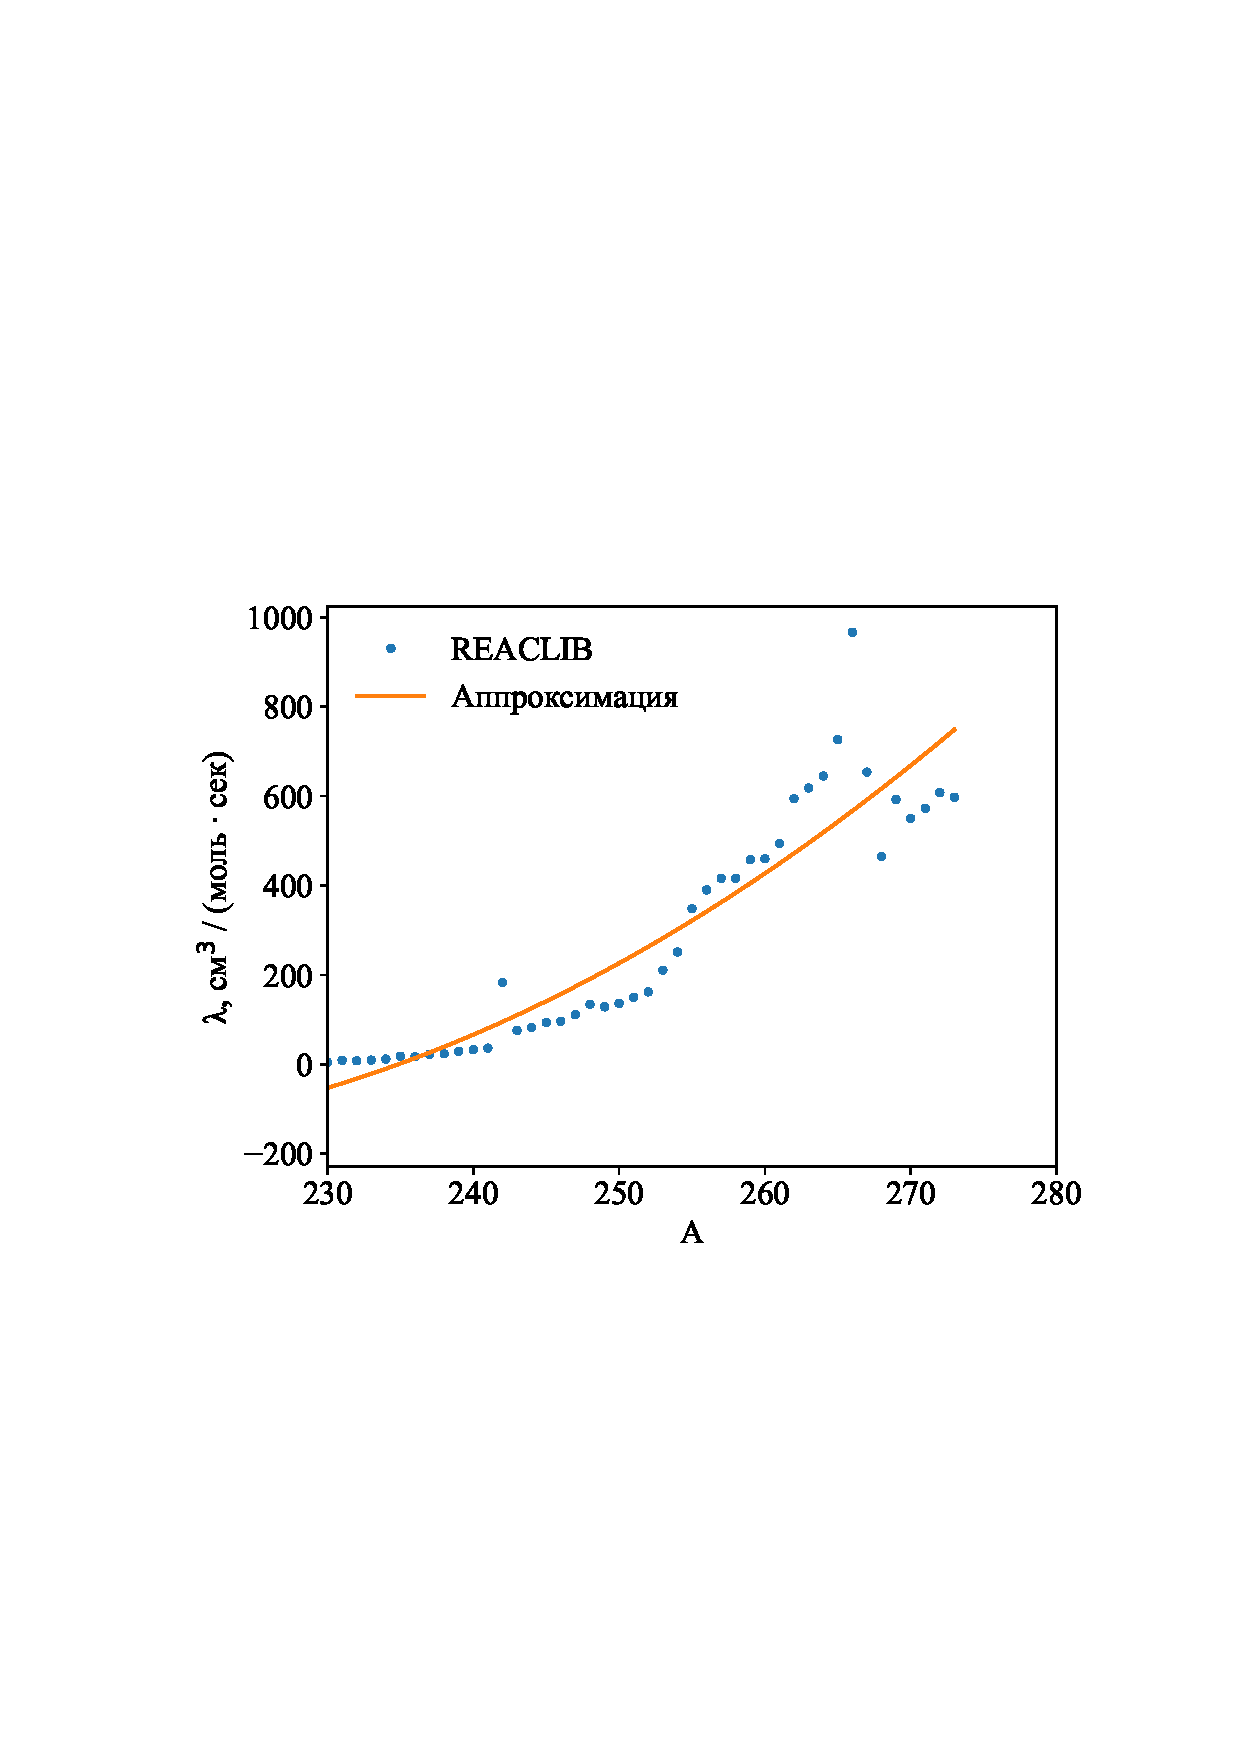
\includegraphics[width=\textwidth]{pics/decay_fit82.pdf}
    \caption{Свинец}
  \end{subfigure}
  \caption{Экстраполяция скоростей слабых распадов для нейтроноизбыточных ядер на основе данных из библиотеки REACLIB двумя модельными функциями: полиномом второй степени и формулой скорости $\beta$-распада на основе правила Сарджента и формулы Вайцзеккера.}
  \label{img:weak_decay_fit}
\end{figure}

  

  Нами также рассматривалась более качественная модельная функция, использующая правило Сарджента $\lambda \sim Q^5$, где энерговыделение $Q$ можно было бы связать с массовым числом $A$ через формулу Вайцзеккера для энергии связи. Такая аппроксимация менее удобна из-за большего числа параметров, а существенного выигрыша в точности не дает. Кроме того, следует учесть, что с приближением к границе существования ядер обычный $\beta^-$-распад начинает подавляться слабыми распадами с вылетом двух и трех нейтронов. Учесть это обстоятельство в качественной модельной функции было бы затруднительно. Поэтому в итоге мы остановились на простейшей экстраполяции полиномом второй степени. Результаты экстраполяции скоростей $\beta^-$-распада для нейтроноизбыточных изотопов тербия и свинца представлены на рис.~\ref{img:weak_decay_fit}.

  Отметим, что и в REACLIB, и в различных таблицах теоретических масс ядер дополнительно представлены данные для изотопов вне области существования ядер, находящиеся вблизи границ отделения протона и нейтрона. Эти данные не являются избыточными, так как позволяют учитывать, что под воздействием интенсивных нейтронных захватов ядро все таки может выйти за границу отделения и просуществовать там некоторое время.   
